% \vspace{-0.5cm}
\section{Quantitative Analysis}
\label{sec:evaluation}

% In this section, we aim to evaluate the selected approaches in three aspects using our evaluation framework: 
% 1) How effective are the selected approaches under different experimental settings? 
% 2) How robust are the selected approaches against evolution, obfuscation, and adversarial attacks? 
% 3) How efficient are the selected approaches in terms of feature transformation and ML modeling?
% We also provide a detailed analysis of the results to gain a deeper understanding of the current state-of-the-art in Android malware detection.

% In this section, we conduct a quantitative analysis of the selected approaches using \codename.

% \jh{One of the primary contributions of our study is conducting a comprehensive quantitative analysis of the selected representative approaches.
% This analysis aims to demonstrate and unravel the impacts on the performance of various application scenarios, \textit{e.g.,} different malware ratios and adversarial attacks, thereby providing a clue to the current state of ML-based Android malware detection.
% }

%
% This analysis aims to estimate and unravel the effects of various experimental settings, such as different data sizes, goodware-to-malware ratios, and the presence of adversarial attacks, on the performance of these methods.
% Such experiments offer valuable insights into the current state of ML-based Android malware detection.
% Specifically, we re-implement these approaches using our general-purpose framework, \codename.
% We then assess their effectiveness, robustness, and efficiency on our crafted dataset.

% One of our contributions is conducting a quantitative analysis of the selected approaches.
This analysis seeks to assess and disentangle the effects of various experimental settings --- such as data size, goodware-to-malware ratios, and the presence of adversarial attacks --- on the performance of these methods.
By conducting these experiments, we can observe how current ML-based Android malware detection methods perform under varied conditions and identify key factors that contribute to an effective malware detector.
Specifically, we re-implement the 12 representative approaches outlined in Sec.~\ref{sec:approach_analysis} using our general-purpose framework
(Implementation details are in Appendix~\ref{sub:approach_overview}).
We then evaluate their effectiveness (Sec.~\ref{effectiveness}), robustness (Sec.~\ref{robustness}), and efficiency (Sec.~\ref{efficiency}) on a large-scale, long-duration dataset (Sec.~\ref{sec:dataset}) tailored for this study.

% In this section, we re-implement the 12 methods described in Section~\ref{sec:approach_analysis} and assess their effectiveness, robustness, and efficiency on our curated dataset (more reproduction details are provided in~\ref{sub:approach_overview}).
% Through this, we aim to provide a comprehensive understanding of the state-of-the-art techniques in Android malware detection.
% \subsection{\codename}
% \label{sec:framework}

% % \jiahao{Add more discussion and illustration of the framework. How to use it? What are the key components?}
% Figure~\ref{fig:framework} illustrates the workflow of \codename.
% The procedure initiates with a collection of apps, from which a set of features is extracted and stored in a feature database.
% These features are then processed by a preprocessor, being transformed into a numerical vector.
% After that, an ML model is trained and evaluated for detecting malware.
% \codename is also equipped with adaptable experimental settings to support multiple real-world scenarios. 
% It is implemented in 17K lines of Python code, detailed in supplementary materials~\cite{supplementary}.

% % The framework is crafted with two guiding principles at its core: modularization and flexibility.
% % \jh{\codename is modular, which makes it easy to extend and customize according to various requirements.}
% % This is achieved by decoupling it into three modules: \textit{feature database}, \textit{preprocessor}, and \textit{ML model}.
% % Given the structured format of the \textit{feature database}, one can easily incorporate new features and integrate them into the assessment pipeline.
% % Moreover, the \textit{preprocessor} can be tailored to accommodate various approaches, granting users the flexibility to determine what/how features are used.
% % The \textit{ML model} is preloaded with various ML models, such as SVM, MLP, CNN, and AE.
% % Alternatively, \codename also supports custom models, allowing users to incorporate their own models into the framework.
% % Given the structured format of the \textit{feature database} (details can be found in~\ref{sub:feature_db}), one can easily incorporate new features and integrate them into the assessment pipeline.
% \codename consists of three modules: \textit{feature database}, \textit{preprocessor}, and \textit{ML model}.
% % This modular design simplifies the development of ML-based Android malware detectors.
% \textit{Feature database} organizes the extracted features categorically, including Manifest, ProgramGraph, DisassembledCode, and SharedLibrary, which can be easily extended to incorporate new features.
% \textit{Preprocessor} is used to retrieve and encode features before feeding them into \textit{ML model}.
% % This module can be tailored to support different detectors, granting flexibility in feature selection and usage.
% % The role of \textit{preprocessor} is to transform (\textit{i.e.,} retrieve and encode) APK features and can be tailored to suit various malware detectors, granting flexibility in feature selection and usage.
% % The \textit{ML model} is preloaded with various ML models, such as SVM, MLP, and AE.
% % Additionally, it offers the capability for model customization, enabling users to easily integrate their own models into the framework.
% \textit{ML model} integrates widely used ML models, \textit{e.g.,} RF, SVM, KNN, MLP, LSTM, CNN, GNN, and AE.
% It also supports model customization --- for example, one can easily add new neural networks of different architectures.
% % It also supports model customization, making it straightforward to incorporate bespoke models. 
% % To develop a new detector, one only needs to customize \textit{preprocessor} to select corresponding features from \textit{feature database} and feed them into \textit{ML model}.

% \codename provides configurable experimental settings to support different scenarios.
% Parameters, such as goodware-to-malware ratios and training data sizes, are all adjustable.
% Different configurations enable the creation of diverse evaluation scenarios.
% % This capability enhances the app selection process, enabling the creation of diverse evaluation scenarios. 
% % This facilitates app selection to construct diverse scenarios, ensuring comprehensive and accurate evaluation.
% \codename also includes an APK obfuscator~\cite{aonzo2020obfuscapk}, which can produce different types of obfuscated samples, \textit{e.g.,} code modification and identifier renaming.
% Moreover, this framework incorporates an adversarial samples generation mechanism from AndroidHIV~\cite{chen2019android}, allowing the assessment of models' resilience to adversarial attacks.

% \subsection{\codename Implementation}
% \codename is developed in 17K lines of Python code.
% To ensure consistency and mitigate biases from different feature extraction toolchains and learning frameworks, we adopt standardized techniques across all tasks.
% For feature extraction, we use Androguard~\cite{androguard} to disassemble APK files and derive features such as permissions, intents, and program graphs. 
% LibRadar~\cite{libradar} helps in identifying third-party libraries within the applications, while Angr~\cite{angr} is used for analyzing native libraries and capturing essential features like opcodes and API calls. 
% When it comes to ML models, the scikit-learn library is our choice for traditional ML algorithms like SVM, KNN, and RF.
% On the other hand, for DL architectures such as CNN, GNN, and AE, we resort to Pytorch~\cite{pytorch}.
% This uniform approach ensures a balanced evaluation, concentrating purely on the uniqueness and performance of each method.

% \codename also includes an APK obfuscator~\cite{aonzo2020obfuscapk}, which can produce different types of obfuscated samples, \textit{e.g.,} code modification and identifier renaming.
% Moreover, this framework incorporates an adversarial samples generation mechanism from AndroidHIV~\cite{chen2019android}, allowing the assessment of models' resilience to adversarial attacks.
\subsection{Dataset}
\label{sec:dataset}
\subsubsection{\textbf{Primary Dataset}}
\label{primary_dataset}
For an evaluation that mirrors real-world scenarios and supports a multi-dimensional assessment, it is crucial that the dataset adheres to the following criteria~\cite{pendlebury2019tesseract}.
\textit{Market Diversity}:
Android apps are distributed across various app stores; it is better to sample them from multiple platforms to ensure comprehensive representation.
We choose to collect our dataset from AndroZoo~\cite{allix2016androzoo}, which is a growing collection of apps from different platforms, like Google Play, PlayDrone, VirusShare, and AppChina.
\textit{Grayware}:
Owing to the uncertain nature of grayware, incorporating it might skew the results.
To filter out grayware, we use the number of positive antivirus alerts (denoted as $p$) derived from VirusTotal~\cite{virustotal} as a criterion.
Following previous studies~\cite{pendlebury2019tesseract,miller2016reviewer}, apps with $p\geq 4$ are categorized as malicious, while those with $p=0$ are considered benign.
\textit{Time Distribution}:
To study malware evolution~\cite{cai2020assessing,lei2019evedroid}, the dataset should cover a wide range of years.
We set the time span as ten years for a comprehensive evaluation.
However, during app collection, we find that due to collection delays, the number of malware samples in the last few years is relatively small, making it challenging to support a thorough evaluation~\cite{arp2022and}.
Therefore, similar to previous studies~\cite{chen2023continuous,gao2024comprehensive}, we collect apps from 2011 to 2020.
\tosem{Highlight the apps are enough.}
\textit{Malware Ratio}:
To mimic actual conditions, we select apps based on a monthly time window, ensuring that around 2,000 apps are collected each month, with a goodware-to-malware ratio aligning with the estimated $9:1$ in the wild~\cite{pendlebury2019tesseract}.
% Additionally, to ensure the quality of the dataset, we exclude apps that fail to be analyzed by AndroGuard~\cite{androguard}.
Additionally, to ensure the quality of the dataset, we exclude apps that cannot be parsed by AndroGuard~\cite{androguard} because we cannot extract the required features for malware detection.
\tosem{Provide a more detailed explanation of the deduplication process.}

Finally, we obtain a dataset of 221,310 Android apps, i.e., 22,870 malicious and 198,440 benign apps, as summarized in Table~\ref{tab:dataset_stat}.

\begin{table}[t]
    \renewcommand{\arraystretch}{0.9}
    \centering
    \caption{Evaluation Dataset Statistics.
    The unit used for measuring APK size is megabytes (MB).}
    % \vspace{-0.1cm}
    \begin{adjustbox}{width=0.7\linewidth, center}
    \begin{tabular}{c|ccccc}
    \hline
    \textbf{Year}  & \textbf{Malicious} & \textbf{Benign} & \textbf{M+B} & \textbf{M/(M+B)} & \textbf{Avg.Size} \\ \hline
    \textbf{2011}  & 2,085   & 17,878   & 19,963& 10.4\%& 2.26   \\
    \textbf{2012}  & 2,137   & 18,687   & 20,824& 10.3\%& 3.58   \\
    \textbf{2013}  & 2,182   & 18,631   & 20,813& 10.5\%& 5.21   \\
    \textbf{2014}  & 2,346   & 20,142   & 22,488& 10.4\%& 6.91   \\
    \textbf{2015}  & 2,369   & 20,643   & 23,012& 10.3\%& 9.52   \\
    \textbf{2016}  & 2,390   & 21,292   & 23,682& 10.1\%& 12.26  \\
    \textbf{2017}  & 2,389   & 21,006   & 23,395& 10.2\%& 16.24  \\
    \textbf{2018}  & 2,326   & 20,099   & 22,425& 10.4\%& 16.62  \\
    \textbf{2019}  & 2,345   & 20,260   & 22,605& 10.4\%& 17.27  \\
    \textbf{2020}  & 2,301   & 19,802   & 22,103& 10.4\%& 16.65  \\ \hline
    \textbf{Total} & 22,870  & 198,440  & 221,310      & 10.3\%& 10.86  \\ \hline
    \end{tabular}
    \end{adjustbox}
    \label{tab:dataset_stat}
    \vspace{-0.3cm}
\end{table}

\begin{table}[h]
    \centering
    \caption{Data distribution of four sub-datasets. M/N indicates M benign and N malicious apps.}
    % \vspace{-0.1cm}
    \begin{adjustbox}{width=0.53\linewidth, center}
 \begin{tabular}{r|r|r|c}
     \hline
     \multicolumn{1}{c|}{\textbf{Training}} & \multicolumn{1}{c|}{\textbf{Validation}} & \multicolumn{1}{c|}{\textbf{Testing}} & \textbf{Alias} \\ \hline
     \multirow{2}{*}{14,400/1,600}    & 1,800/200    & 1,800/200 & \ding{182}  \\ \cline{2-4} 
   & 1,000/1,000  & 1,000/1,000      & \ding{183}  \\ \hline
     \multirow{2}{*}{8,000/8,000}     & 1,800/200    & 1,800/200 & \ding{184} \\ \cline{2-4} 
   & 1,000/1,000  & 1,000/1,000      &  \ding{185}\\ \hline
     \end{tabular}
    \end{adjustbox}
    \label{tab:effectiveness_dataset}
    \vspace{-0.3cm}
\end{table}

\bulletpoint{Settings}
To support certain evaluation scenarios, we construct four sub-datasets from the aforementioned dataset.
For each sub-dataset, apps are randomly sampled to form training, validation, and testing sets.
Table~\ref{tab:effectiveness_dataset} shows their data distribution.
Importantly, the apps in these sub-datasets are sampled from different years to ensure comprehensive representation.
For instance, for \ding{182}, each year contributes 1440 benign and 160 malicious apps for training, 180 benign and 20 malicious apps for validation, and the same for testing. 
Duplicate apps are also avoided across these sets.

\subsubsection{\textbf{Additional Dataset}}
\label{additional_dataset}
\tosem{To complementary verify the application of our framework, \codename, we also collect apps recently from 2021 to 2024, although the dataset is smaller, to further evaluate exsiting solutions and support our main findings.}

\subsection{Effectiveness}
\label{effectiveness}
In this section, we examine how the effectiveness of the selected approaches varies across different experimental settings to pinpoint the factors that contribute to an effective malware detector. 
Specifically, we focus on the following aspects: goodware-to-malware ratio, training set size, APK features, and model selection.
These factors are pivotal as they influence the quality of the training data and the model's ability to extract relevant information, both of which are essential for the performance of ML-based detectors.

\begin{table}[t]
    \centering
    \renewcommand{\arraystretch}{0.9}
    \caption{The effectiveness of the approaches across varied goodware-to-malware ratios in training and testing sets.}
    % \vspace{-0.1cm}
    \begin{adjustbox}{width=0.74\linewidth, center}
 \begin{tabular}{@{}c|cccc|cccc@{}}
     \toprule
     \multirow{3}{*}{\textbf{\begin{tabular}[c]{@{}c@{}}\\Selected\\ Approach\end{tabular}}} & \multicolumn{4}{c|}{\textbf{B:M=9:1 in Tr (\ding{182} - \ding{183})}}& \multicolumn{4}{c}{\textbf{B:M=1:1 in Tr (\ding{184} - \ding{185})}}\\ \cmidrule(l){2-9} 
     & \multicolumn{2}{c|}{\textbf{B:M=9:1 in Ts}}& \multicolumn{2}{c|}{\textbf{B:M=1:1 in Ts}}& \multicolumn{2}{c|}{\textbf{B:M=9:1 in Ts}}& \multicolumn{2}{c}{\textbf{B:M=1:1 in Ts}} \\ \cmidrule(l){2-9} 
     & \multicolumn{1}{c|}{\textbf{F1}} & \multicolumn{1}{c|}{\textbf{Acc.}} & \multicolumn{1}{c|}{\textbf{F1}} & \textbf{Acc.} & \multicolumn{1}{c|}{\textbf{F1}} & \multicolumn{1}{c|}{\textbf{Acc.}} & \multicolumn{1}{c|}{\textbf{F1}} & \textbf{Acc.} \\ \midrule
     Drebin & \multicolumn{1}{c|}{0.722}& \multicolumn{1}{c|}{\textbf{0.948}} & \multicolumn{1}{c|}{0.791}& 0.823 & \multicolumn{1}{c|}{0.650}& \multicolumn{1}{c|}{0.901} & \multicolumn{1}{c|}{0.918}& 0.917 \\ \midrule
     MamaDroid& \multicolumn{1}{c|}{0.661}& \multicolumn{1}{c|}{0.945} & \multicolumn{1}{c|}{0.693}& 0.763 & \multicolumn{1}{c|}{0.650}& \multicolumn{1}{c|}{0.902} & \multicolumn{1}{c|}{0.895}& 0.897 \\ \midrule
     Mclaughlin et al.& \multicolumn{1}{c|}{0.714}& \multicolumn{1}{c|}{0.946} & \multicolumn{1}{c|}{0.799}& 0.828 & \multicolumn{1}{c|}{0.682}& \multicolumn{1}{c|}{\textbf{0.924}} & \multicolumn{1}{c|}{0.916}& 0.916 \\ \midrule
     HinDroid & \multicolumn{1}{c|}{\textbf{0.731}}& \multicolumn{1}{c|}{0.943} & \multicolumn{1}{c|}{0.819}& 0.842 & \multicolumn{1}{c|}{\textbf{0.701}}& \multicolumn{1}{c|}{0.924} & \multicolumn{1}{c|}{\textbf{0.925}}& \textbf{0.925} \\ \midrule
     DeepRefiner & \multicolumn{1}{c|}{0.657}& \multicolumn{1}{c|}{0.932} & \multicolumn{1}{c|}{0.776}& 0.809 & \multicolumn{1}{c|}{0.667}& \multicolumn{1}{c|}{0.918} & \multicolumn{1}{c|}{0.881}& 0.881 \\ \midrule
     Kim et al.& \multicolumn{1}{c|}{\textbf{0.782}}& \multicolumn{1}{c|}{\textbf{0.952}} & \multicolumn{1}{c|}{\textbf{0.907}}& \textbf{0.912} & \multicolumn{1}{c|}{\textbf{0.753}}& \multicolumn{1}{c|}{0.\textbf{941}} & \multicolumn{1}{c|}{\textbf{0.938}}& \textbf{0.937} \\ \midrule
     MalScan& \multicolumn{1}{c|}{0.684}& \multicolumn{1}{c|}{0.939} & \multicolumn{1}{c|}{0.793}& 0.823 & \multicolumn{1}{c|}{0.587}& \multicolumn{1}{c|}{0.877} & \multicolumn{1}{c|}{0.880}& 0.880 \\ \midrule
     SDAC& \multicolumn{1}{c|}{0.522}& \multicolumn{1}{c|}{0.916} & \multicolumn{1}{c|}{0.627}& 0.720 & \multicolumn{1}{c|}{0.524}& \multicolumn{1}{c|}{0.850} & \multicolumn{1}{c|}{0.845}& 0.844 \\ \midrule
     HomDroid & \multicolumn{1}{c|}{\textbf{0.734}}& \multicolumn{1}{c|}{\textbf{0.949}} & \multicolumn{1}{c|}{0.816}& 0.841 & \multicolumn{1}{c|}{\textbf{0.701}}& \multicolumn{1}{c|}{\textbf{0.925}} & \multicolumn{1}{c|}{0.912}& 0.914 \\ \midrule
     Xmal& \multicolumn{1}{c|}{0.698}& \multicolumn{1}{c|}{0.942} & \multicolumn{1}{c|}{0.826}& \textbf{0.847} & \multicolumn{1}{c|}{0.674}& \multicolumn{1}{c|}{0.916} & \multicolumn{1}{c|}{\textbf{0.923}}& \textbf{0.924} \\ \midrule
     RAMDA& \multicolumn{1}{c|}{0.636}& \multicolumn{1}{c|}{0.905} & \multicolumn{1}{c|}{\textbf{0.841}}& \textbf{0.852} & \multicolumn{1}{c|}{0.510}& \multicolumn{1}{c|}{0.829} & \multicolumn{1}{c|}{0.871}& 0.865 \\ \midrule
     MSDroid& \multicolumn{1}{c|}{0.648}& \multicolumn{1}{c|}{0.919} & \multicolumn{1}{c|}{\textbf{0.834}}&0.828 & \multicolumn{1}{c|}{0.522}& \multicolumn{1}{c|}{0.853} & \multicolumn{1}{c|}{0.867}& 0.858 \\ \bottomrule
     \end{tabular}
    \end{adjustbox}
    \label{tab:res_ratio}
    \begin{tablenotes}[flushleft, labelsep=0]
 \footnotesize
 \item \textit{Tr:} training set, \textit{Ts:} testing set. \ding{182} - \ding{185} correspond to the four scenarios in Table~\ref{tab:effectiveness_dataset}. The top 3 results for each scenario are highlighted in bold.
 \end{tablenotes}
    \vspace{-0.5cm}
\end{table}

% We investigate how various factors --- goodware-to-malware ratio in training and testing sets, training set size, and APK feature --- affect the effectiveness of these approaches.

\bulletpoint{Goodware-to-malware ratio}
The effectiveness of ML-based Android malware detectors is heavily influenced by malware distributions in the training and testing sets.
Here, we consider two ratios, \textit{i.e.}, 10\%, and 50\%, in both training and testing sets.
These choices are inspired by the estimated 10\% in the wild~\cite{pendlebury2019tesseract} and the 50\% widely used in previous studies~\cite{wu2019malscan,li2021robust,mariconti2016mamadroid}.
The \ding{182} - \ding{185} in Table~\ref{tab:effectiveness_dataset} present these four scenarios.  

Table~\ref{tab:res_ratio} summarizes the results in terms of F1-score and Accuracy.
The results are arranged from left to right, mapping scenarios \ding{182} to \ding{185}.
We observe that all the approaches produce promising results under scenario \ding{185}, characterized by a \texttt{1:1} goodware-to-malware ratio in both training and testing sets.
This demonstrates that these approaches can effectively detect Android malware under ideal conditions, where goodware and malware are balanced.
However, when the malware ratio is adjusted to 10\% (\ding{182}), there is a marked decline in the F1-score across all methods.
% It is evident that most of these approaches suffer from performance degradation when faced with a realistic malware ratio.
% This is primarily due to the limited number of malware samples available for training, which hampers the model's ability to learn effective patterns.
% Additionally, by increasing the malware ratio in testing sets from 10\% to 50\% (\ding{183} and \ding{185}), we notice the F1-scores increase for all methods.
% This is expected, as the increased number of malware samples in the testing set makes models more likely to encounter familiar patterns, leading to improved performance.
% For a coarse and aggregate analysis, upon analyzing the top three results, we find that DL-based approaches appear to outperform TML-based methods when the malware ratio is 50\% (\ding{183} and \ding{185}) --- almost all the top three results are achieved by DL-based methods.
% While in more realistic scenarios (\ding{182} and \ding{184}), DL-based approaches do not exhibit a marked advantage over TML-based methods.
It is evident that many existing approaches experience performance degradation when evaluated under realistic malware ratios.
This is primarily attributed to the scarcity of malware samples in the training data, which constrains the model's ability to learn discriminative malware semantics.
Moreover, when the malware ratio in the test set is increased from 10\% to 50\% (\ding{183} and \ding{185}), we observe a consistent improvement in F1-scores across all methods.
This trend is expected, as a higher prevalence of malware samples in the test set increases the likelihood that models will encounter patterns similar to those seen during training, enhancing their predictive performance.
In a coarse-grained, average analysis, where the influence of differing feature combinations is partially mitigated due to the diverse features used by both TML-based and DL-based approaches, we find an interesting phenomenon: DL-based approaches appear to outperform TML-based methods when the testing malware ratio is 50\% (\ding{183} and \ding{185}) --- almost all the top three results are achieved by DL-based methods.
While in more realistic scenarios (\ding{182} and \ding{184}), DL-based approaches do not exhibit a marked advantage over TML-based methods.
One possible explanation is that DL-based methods are better equipped to capture the complex semantics underlying app behaviors, which tend to be more prominent in datasets with a higher malware ratio.

\tosem{Add more metrics of recall and precision of table 5.}

% This is because malware samples are typically more diverse and intricate, presenting greater challenges for detection.

\bulletpoint{Training set size}
The training set's size is a critical determinant of the effectiveness of ML classifiers~\cite{sun2017revisiting}, since high-quality training data typically provides richer semantic information about malware, which is essential for learning effective classifiers.
However, securing a large, high-quality training set is often infeasible due to the significant costs of data collection and labeling.
% Thus, we experiment with varying training set sizes to simulate different levels of semantic richness. 
% This assumption is justified by the fact that, as more data is included, a broader spectrum of malware semantics is likely to be captured, since our dataset is collected from multiple sources and spans a wide range of years, reflecting the real-world distribution of Android apps.
Thus, we experiment with different training set sizes to simulate varying levels of semantic richness (\textit{i.e.,} larger datasets are assumed to encompass more diverse malware semantics) and analyze their impact on classifier performance.
Specifically, we consider two training set sizes, 50\% and 10\% of the original training set size, while maintaining the malware ratio at 10\%.
% To study the impact of training set size, we down-sample the training set in Table~\ref{tab:effectiveness_dataset}(\ding{182}) to 50\% and 10\% of its initial size, while ensuring that the malware ratio remains 10\%.

Figure~\ref{fig:training_size} shows how these detectors' performance changes when the training set size or semantic richness is reduced.
We normalize the F1-scores of these methods based on their performance obtained with the entire original dataset.
The detailed results are provided in the Appendix~\ref{sec:additional_results}.
The figure clearly shows that reducing the training set size leads to performance degradation across all approaches, underscoring more data enhances capturing malicious patterns.
Interestingly, Mclaughlin et al. and DeepRefiner display a greater sensitivity to training set size compared to others.
One explanation is that, unlike other methods that heuristically select features from apps, these two approaches take the original apps' bytecode as input and automatically extract semantics, requiring more data to learn patterns from raw data as opposed to hand-crafted features.
This finding highlights that the effectiveness of malware detectors is closely tied to the quality of the training data and the semantic richness it provides.
Also, it suggests that heuristic selected features that are semantically rich can be more effective than raw data in scenarios where data is limited.


% {\bf This finding highlights the importance of feature selection in ML-based Android malware detection, especially in scenarios where data is limited.} The features selected needs to be related to the semantics of malware, where further work is needed to quantify the relevance. We also carry out an analysis on how the level of relevance in semantics affects effectiveness. 

% \tdsc{It's better to have a conclusion for Sec. 5.3.}




\begin{figure}[t]
    \centering
    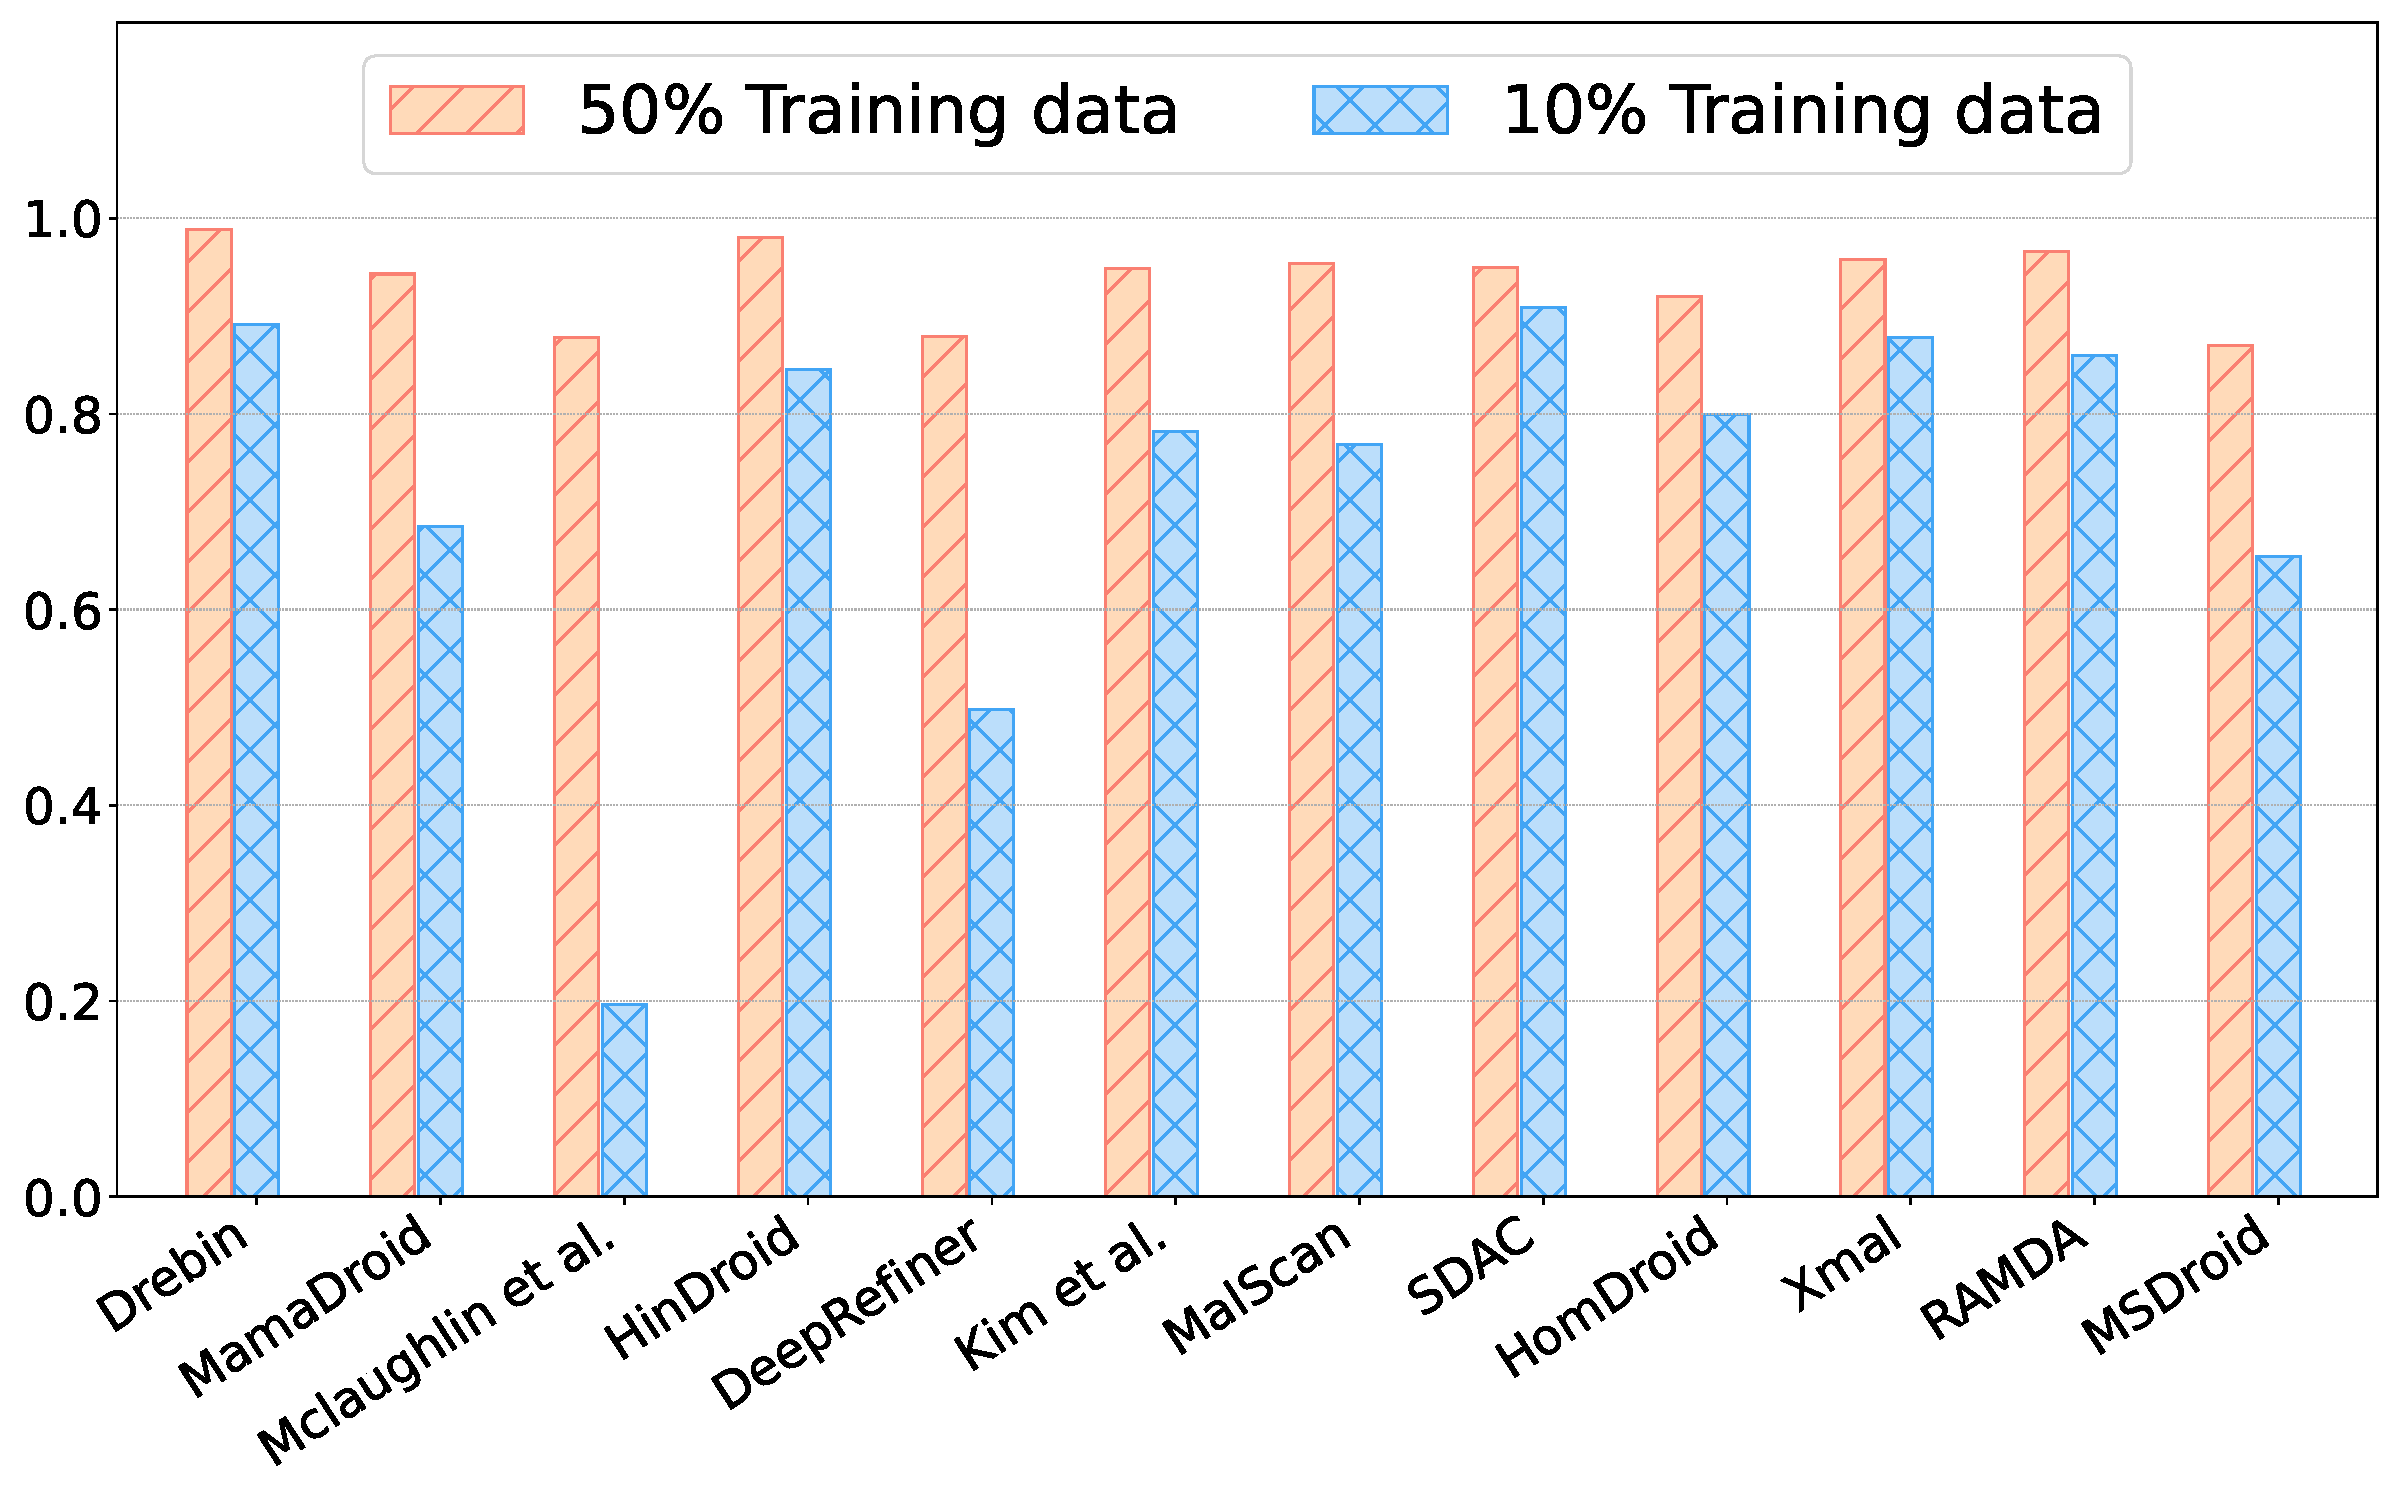
\includegraphics[width=0.64\linewidth]{fig/training_size.pdf}
    \vspace{-0.2cm}
    \caption{Effectiveness of the selected approaches using different sizes of training data.}
    \label{fig:training_size}
    \vspace{-0.5cm}
\end{figure}

% \subsection{Effectiveness vs. Semantics Levels\tdsc{(Domain Semantics?)}}

\bulletpoint{APK feature}
Android malware detectors often leverage diverse features to enhance detection performance~\cite{arp2014drebin,kim2018multimodal,li2021robust}.
The reason is that each feature contributes to characterizing APKs, encoding their unique semantics.
One question arises: does the incorporation of more features necessarily enhance a detector's performance?
To investigate this, we remove individual features from the original feature set to assess the resulting performance.
For this experiment, it is essential that the features of the chosen approaches are decomposable, allowing the sequential removal of individual features.
Accordingly, we spotlight Drebin, Kim et al., Xmal, and RAMDA, owing to their decomposable feature sets.
We exclude methods whose features are highly intertwined.
For instance, MamaDroid and MalScan rely on specific API calls to extract features from program graphs, making it challenging to remove individual features --- if API calls are removed, the graph features will also be removed.

Table~\ref{tab:combination_feats} presents the outcomes of this experiment.
From the table, we observe that Drebin, Xmal, and RAMDA have performance degradation when one feature is removed.
Interestingly, Kim et al. deviate from this trend.
In fact, even after omitting several features, its performance exceeds the original results.
These two observations underscore:
(i) each feature contains unique semantics describing the APKs and contributes to the overall effectiveness of a malware detector, and (ii) the semantics of different feature sets are not always complementary, and merely expanding the feature set does not guarantee enhanced performance.
This phenomenon underscores the importance of evaluating and justifying the inclusion of each feature in a malware detector based on the semantics.

\tosem{Add experiments for Kim, training epoch, and hidden size dimension.}

% These two observations underscore that each feature contributes to the overall effectiveness of a malware detector.
% While in some cases, merely expanding the feature set does not guarantee enhanced performance.

% {\bf This phenomenon underscores the importance of evaluating and justifying the inclusion of each feature in a malware detector based on the semantics.}

\begin{table}[t]
    \centering
    \renewcommand{\arraystretch}{0.8}
    \caption{The impact of APK features on the effectiveness of Drebin, Kim et al., Xmal, and RAMDA.}
    % \vspace{-0.1cm}
    \begin{adjustbox}{width=0.86\linewidth, center}
 \begin{tabular}{@{}l|cc|cc|cc|cc@{}}
 \toprule
 \multirow{2}{*}{\textbf{\raisebox{-0.2cm}{\begin{tabular}[c]{@{}l@{}}Feature\\ Combination\end{tabular}}}} & \multicolumn{2}{c|}{\textbf{Drebin}}      & \multicolumn{2}{c|}{\textbf{Kim et al.}}  & \multicolumn{2}{c|}{\textbf{Xmal}} & \multicolumn{2}{c}{\textbf{RAMDA}} \\ \cmidrule(l){2-9} 
 & \multicolumn{1}{c|}{\textbf{F1}} & \textbf{Acc.} & \multicolumn{1}{c|}{\textbf{F1}} & \textbf{Acc.} & \multicolumn{1}{c|}{\textbf{F1}} & \textbf{Acc.} & \multicolumn{1}{c|}{\textbf{F1}} & \textbf{Acc.} \\ \midrule
 Original   & \multicolumn{1}{c|}{\textbf{0.722}}& \textbf{0.948}  & \multicolumn{1}{c|}{0.726}& 0.944  & \multicolumn{1}{c|}{\textbf{0.698}}& \textbf{0.942}  & \multicolumn{1}{c|}{\textbf{0.636}}& \textbf{0.905}  \\ \midrule
 w/o hardware& \multicolumn{1}{c|}{0.717}& 0.947  & \multicolumn{1}{c|}{0.728}& 0.945  & \multicolumn{1}{c|}{N/A}  & N/A    & \multicolumn{1}{c|}{N/A}  & N/A    \\ \midrule
 w/o app-intent & \multicolumn{1}{c|}{0.622}& 0.936  & \multicolumn{1}{c|}{\textbf{0.776}}& \textbf{0.952}  & \multicolumn{1}{c|}{N/A}  & N/A    & \multicolumn{1}{c|}{0.428}& 0.845  \\ \midrule
 w/o permission & \multicolumn{1}{c|}{0.698}& 0.945  & \multicolumn{1}{c|}{0.692}& 0.939  & \multicolumn{1}{c|}{0.566}& 0.926  & \multicolumn{1}{c|}{0.526}& 0.882  \\ \midrule
 w/o api call& \multicolumn{1}{c|}{0.691}& 0.944  & \multicolumn{1}{c|}{0.699}& 0.942  & \multicolumn{1}{c|}{0.639}& 0.930  & \multicolumn{1}{c|}{0.482}& 0.880  \\ \midrule
 w/o opcode & \multicolumn{1}{c|}{N/A}  & N/A    & \multicolumn{1}{c|}{0.724}& 0.942  & \multicolumn{1}{c|}{N/A}  & N/A    & \multicolumn{1}{c|}{N/A}  & N/A    \\ \midrule
 w/o code string& \multicolumn{1}{c|}{0.702}& 0.944  & \multicolumn{1}{c|}{0.725}& 0.945  & \multicolumn{1}{c|}{N/A}  & N/A    & \multicolumn{1}{c|}{N/A}  & N/A    \\ \bottomrule
 \end{tabular}
    \end{adjustbox}
    \label{tab:combination_feats}
    % \centering
    \begin{tablenotes}[flushleft, labelsep=0]
 \footnotesize
 \item \noindent w/o means without. N/A denotes features are not used in the original work.
 \end{tablenotes}
    \vspace{-0.5cm}
\end{table}


\bulletpoint{Model type}
Given specific features that describe app behaviors, different models can be used to extract semantics and detect malware.
The features reflect the richness of the available semantics, while the models determine how effectively these semantics are leveraged.
In this section, we select MamaDroid, HinDroid, and MalScan, which share the same feature set and feature representation, as shown in Table~\ref{tbl:systematization}, to evaluate the impact of different models on the effectiveness of malware detectors.
From the results in Table~\ref{tab:res_ratio} under scenario \ding{182}, we observe that HinDroid outperforms MamaDroid and MalScan.
This suggests that given a fixed feature set, different models demonstrate varying capabilities in extracting semantics and detecting Android malware.

\bulletpoint{Feature and model combination investigation}
\tosem{choose several models, (RF, SVM, KNN, MLP) and evaluated these models with specifc set of features (Hardware component, application component, intent, permission, API call, opcode, code string, resource information).
Point to there are lots of combination of features, and hint that maybe choose specific features for certain kinds of malware is a trend.
}

\begin{conclusionbox}
    \textit{Summary:}
    The effectiveness of ML-based malware detectors is shaped by various factors, such as APK features and model types. At the core of these influences is the richness of semantics embedded in the features and the models' capability to extract and utilize these semantics.
\end{conclusionbox}



% \vspace{-0.1cm}
\subsection{Robustness against real-world scenarios}
\label{robustness}
Previous works~\cite{pendlebury2019tesseract,li2023black,gao2024comprehensive} have started investigating the resilience of detectors when faced with real-world challenges such as malware evolution, obfuscation, and adversarial attacks.
Nonetheless, they often focus on a subset of these challenges or employ unrealistic experimental settings, potentially skewing their findings.
For instance, \textsc{Tesseract}~\cite{pendlebury2019tesseract} explores the impact of malware evolution, while Gao~\cite{gao2024comprehensive} assesses the robustness of detectors using an unrealistic balanced dataset.
This section aims to fill these gaps by thoroughly re-evaluating the robustness of the selected approaches in real-word settings, providing a clearer picture of where ML-based malware detection stands today.

\begin{figure*}[t]
    \centering
    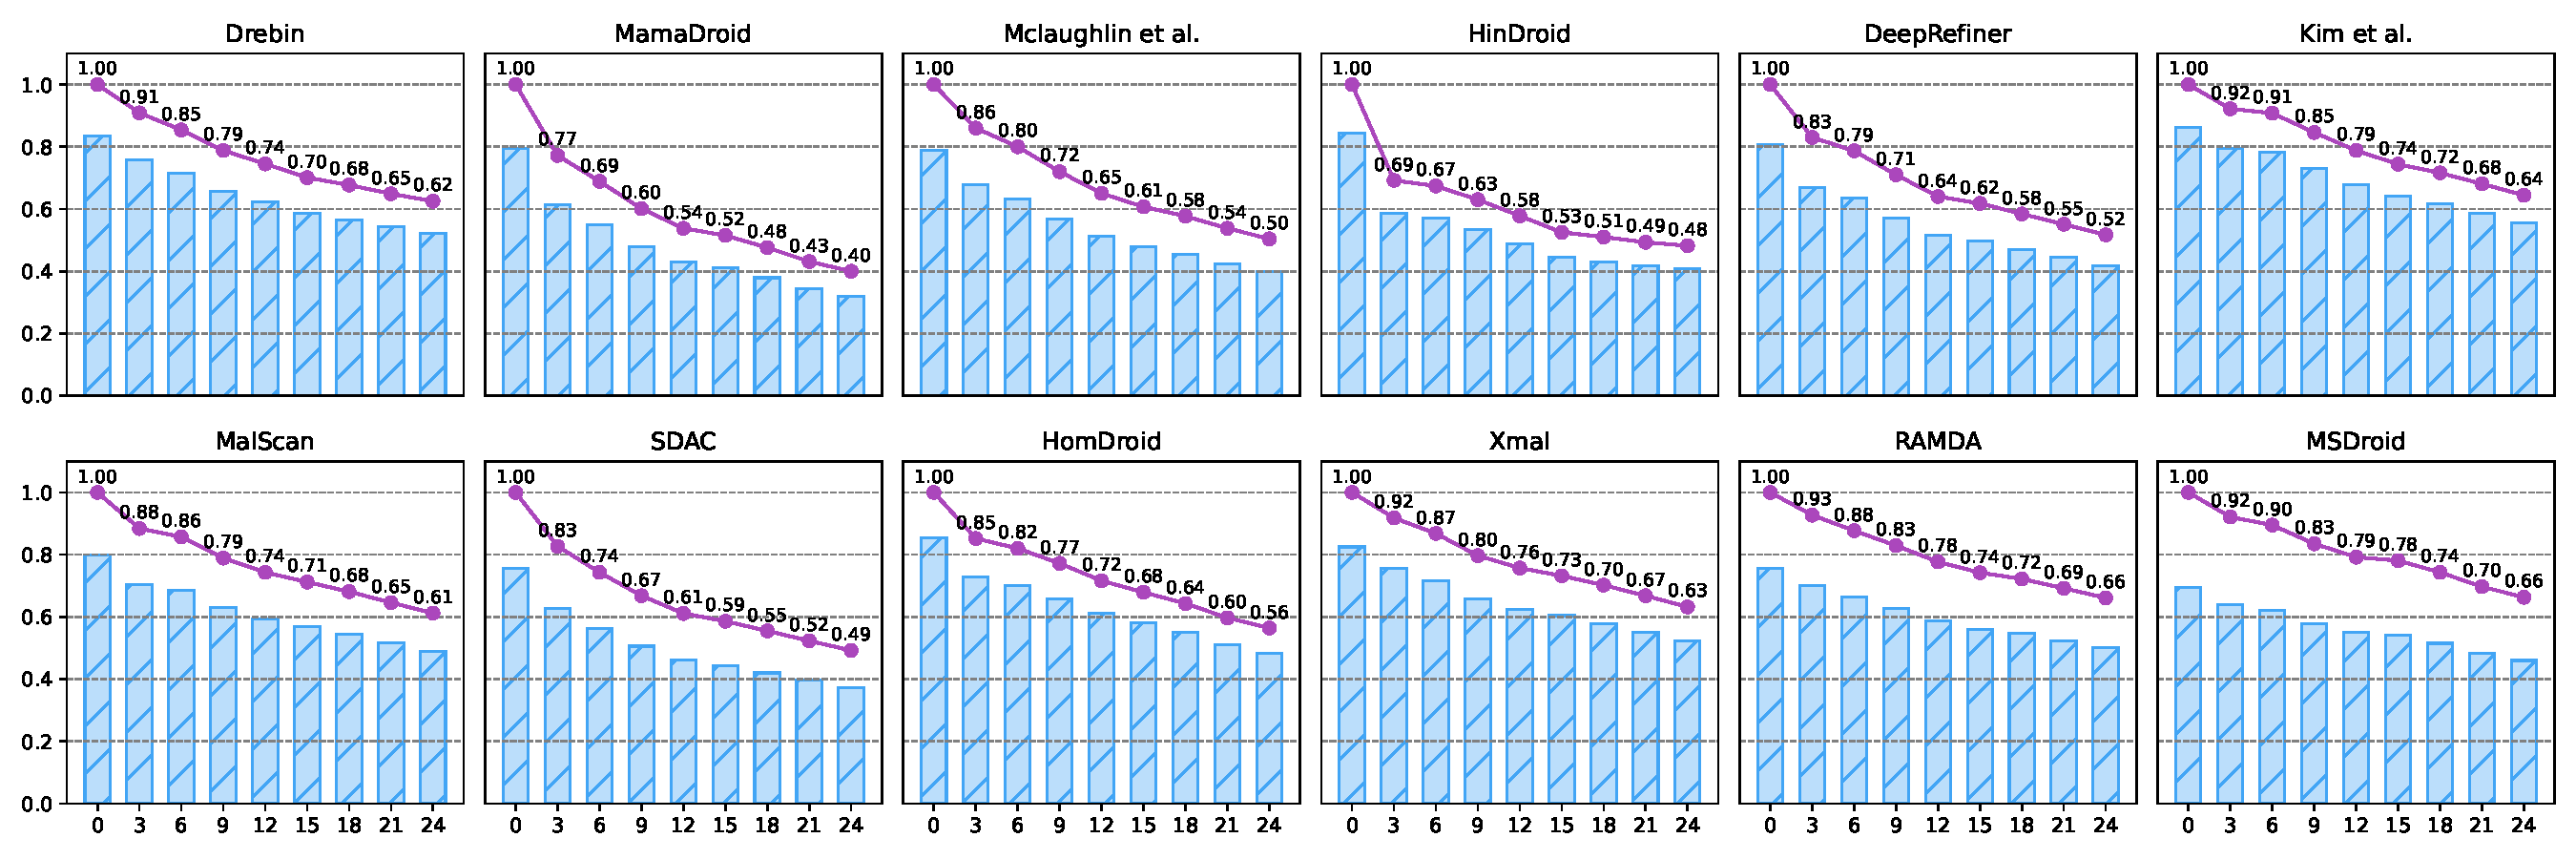
\includegraphics[width=\linewidth]{fig/evolution.pdf}
    % \vspace{-0.1cm}
    \caption{The performance of the selected techniques against diverse malware evolution periods. Columns display the absolute values of $AUT(F1, N)$.
    The line charts depict the relative percentage of $AUT(F1, N)$ against $AUT(F1, 0)$.}
    \label{fig:evolution}
\vspace{-0.3cm}
\end{figure*}

\bulletpoint{Malware evolution}
To quantify the impact of evolution on malware detectors, we utilize the $AUT(f, N)$~\cite{pendlebury2019tesseract}, where $f$ denotes the F1-score of a given approach, and $N$ represents the evolution period. 
The definition of $AUT(f, N)$ can be found in the Appendix~\ref{sub:aut}.
We set $N$ to 3, 6, 9, 12, 15, 18, 21, and 24 months in this experiment.
This metric ranges in (0, 1), where higher values indicate greater resilience to malware evolution.
In the study, we adopt a rolling algorithm over the data from 2011 to 2020 to calculate the $AUT(f, N)$.
Specifically, for each year, from 2011 to 2020, we first partition the data into training, validation, and testing sets with \texttt{8:1:1}.
Next, we train models with the training data, validate to get the best model, and evaluate it on the test set to get the F1-score as $AUT(F1, 0)$.
Then, the model is applied to test data in the next $N$ months, yielding $N$ F1-scores. 
These scores are further used to calculate the $AUT(F1, N)$.
By averaging the $AUT(F1, N)$ values sourced from distinct yearly datasets, we chart the outcomes in Figure~\ref{fig:evolution}.

It is clear that malware evolution affects the effectiveness of these selected techniques.
This is within expectations, as malware evolves over time, the semantics of malware may change, making it harder for detectors to capture these changes.
Most DL approaches display superior resilience against malware evolution compared to their TML counterparts.
Specifically, the majority of DL techniques retain about 60\% effectiveness even after two years. 
In contrast, many TML methods see their F1-scores reduced to 50\% within the same time span.
This disparity can be traced back to the inherent capability of DL methods to discern intricate patterns, which TML might miss.
Interestingly, Mclaughlin et al. and DeepRefiner, do not fare as well over time.
This could be attributed to their reliance on apps' original bytecode as input, which may contain more noise and complicate the semantic extraction process.
\tosem{Add more analysis how to improve the robustness}

\begin{table}[t]
    \centering
    \renewcommand{\arraystretch}{0.7}
    \caption{The F-score of the selected approaches under different obfuscation strategies~\cite{aonzo2020obfuscapk}.}
    % \vspace{-0.1cm}
    \begin{adjustbox}{width=0.74\linewidth, center}
    \begin{tabular}{@{}c|c|c|c|c|c@{}}
    \toprule
    \diagbox[innerleftsep=-0.1em, innerrightsep=-0.3em, height=2.7em,width=7em]{\textbf{Approach}}{\textbf{Obfuscation}} & \textbf{\begin{tabular}[c]{@{}c@{}}Without \\ Obfus.\end{tabular}} & \textbf{\begin{tabular}[c]{@{}c@{}}Rename \\ Identifier\end{tabular}} & \textbf{\begin{tabular}[c]{@{}c@{}}Encrypt \\ Resource\end{tabular}} & \textbf{\begin{tabular}[c]{@{}c@{}}Modify \\ Code\end{tabular}} & \textbf{\begin{tabular}[c]{@{}c@{}}Reflect \\ Invocation\end{tabular}} \\ \midrule
    Drebin      & 0.732 & 0.702 & 0.701 & 0.732 & 0.732 \\ \midrule
    MamaDroid   & 0.653 & 0.274 & 0.449 & 0.150 & 0.461 \\ \midrule
    Mclaughlin et al.  & 0.750 & 0.699 & 0.722 & 0.175 & 0.727 \\ \midrule
    HinDroid    & 0.750 & 0.750 & 0.741 & 0.750 & 0.735 \\ \midrule
    DeepRefiner & 0.692 & 0.618 & 0.658 & 0.297 & 0.612 \\ \midrule
    Kim et al.  & 0.795 & 0.795 & 0.611 & 0.795 & 0.798 \\ \midrule
    MalScan     & 0.675 & 0.675 & 0.675 & 0.681 & 0.687 \\ \midrule
    SDAC & 0.563 & 0.538 & 0.552 & 0.495 & 0.552 \\ \midrule
    HomDroid    & 0.729 & 0.751 & 0.706 & 0.728 & 0.739 \\ \midrule
    Xmal & 0.727 & 0.727 & 0.727 & 0.727 & 0.727 \\ \midrule
    RAMDA& 0.635 & 0.635 & 0.635 & 0.635 & 0.635 \\ \midrule
    MSDroid     & 0.672 & 0.675 & 0.610 & 0.356 & 0.494 \\ \bottomrule
    \end{tabular}
    \end{adjustbox}
    \label{table:res_obfuscation}
    \vspace{-0.3cm}
\end{table}

\bulletpoint{Obfuscation}
Obfuscation techniques often alter an app's code. 
It can also affect the effectiveness of malware detectors~\cite{he2022msdroid}.
This part explores the influences of popular obfuscation techniques, \textit{i.e.,} renaming identifiers, encrypting resources, modifying code, and invoking reflection~\cite{aonzo2020obfuscapk}, on the selected approaches.

We apply the obfuscation strategies discussed earlier to the testing set in Table~\ref{tab:effectiveness_dataset}(\ding{182}).
Only the apps that can be successfully obfuscated by all the strategies are included in the obfuscated testing set, which contains 1,303 apps.
The effectiveness of the selected approaches, previously trained on the original training set, is then evaluated on this obfuscated testing set.
Table~\ref{table:res_obfuscation} summarizes the results.
Clearly, most methods exhibit a performance decrease when subjected to obfuscation.
This is expected, as obfuscation can hidden the malicious semantics, making it harder for detectors to capture them.
Specifically, the impact of obfuscation on detectors significantly depends on how the detectors utilize APK features.
For instance, Xmal and RAMDA show greater robustness against obfuscation.
This is mainly because the employed obfuscation techniques do not change their used features.
In contrast, MamaDroid and MSDroid, relying on the code structure, tend to be more susceptible to the code modification.
This suggests that the impact of obfuscation on detectors is closely related to the degree to which obfuscation techniques alter the semantics of the features utilized by the detectors.
Also, by comparing MamaDroid and MSDroid --- both relying on the code structure --- we observe that a detector's robustness against obfuscation is also shaped by the model's semantic extraction capability.
\tosem{- permission from manifest
- extracted APIs, the list is hardcode, we simiply check the obfuscation, system api, doest not check it.
}


\bulletpoint{Adversarial attack}
We now utilize the dataset from Table~\ref{tab:effectiveness_dataset}(\ding{182}) to explore the impact of adversarial attacks on the performance of these selected approaches.
It is worth noting that we exclude approaches Mclaughlin et al. and DeepRefiner from this experiment.
This is because they truncate features at a certain size, making them easily bypassable.
Attackers can embed malicious code in the ignored part to evade detection.


% Mclaughlin et al. and DeepRefiner are excluded since they truncate features at a certain size, making them easily bypassable.
% Attackers can embed malicious code in the ignored part to evade detection.

To investigate the impact of adversarial attacks, we employ two primary strategies: Jacobian Saliency Map Attack (JSMA) and Randomized Input (RI).
These two techniques are chosen for their simplicity and effectiveness, compromising most ML-based malware detectors, as shown in Table~\ref{tab:adversarial}.
This suggests that more advanced attack strategies could pose even greater threats to these detectors~\cite{he2023efficient,zhao2021structural}.
For JSMA, we first train a substitute model with the training set, followed by applying JSMA to the model to generate adversarial samples.
For RI, we randomly change a certain percentage of features in the testing set to produce adversarial examples.
When crafting adversarial samples, we follow~\cite{li2023black,chen2019android} to ensure the feature modifications are domain-mappable and can be repackaged to APKs.
For feature-vector-based approaches like Drebin, we follow~\cite{chen2019android} by constraining modifications to vector bits that are 0, changing them to 1.
This ensures that all required permissions and functions remain unchanged, keeping the app's functionality unaffected.
For graph-based solutions, we introduce non-disruptive modifications to the graph structures that do not alter the app's functionality.
The graph structure includes non-leaf nodes (user-defined functions) and leaf nodes (Android API). 
When adding a new edge, we select a non-leaf node in the graph and add a try block with a callee chosen from leaf nodes.
Since leaf nodes do not call any other nodes, the added edge does not affect the app's functionality.
% Taking Drebin as an example, we restrict our modifications to changing feature vectors from 0 to 1, keeping apps' functionalities unaffected.
To measure the robustness against adversarial attacks, we use two metrics from~\cite{li2023black}: Adversarial Success Rate (ASR) and Adversarial Perturbation Ratio (APR).
The detailed definitions can be found in the Appendix~\ref{sub:aut}.
Both metrics range (0, 1).
A higher ASR indicates increased vulnerability to adversarial attacks, while a higher APR suggests greater robustness against such attacks due to the model's ability to withstand perturbations.

By analyzing Table~\ref{tab:adversarial}, we note that JSMA yields an average ASR of 98.8\% across the evaluated approaches, indicating their vulnerability to such basic adversarial attacks, let alone more sophisticated ones~\cite{he2023efficient}.
The employed strategies are less effective on MamaDroid, HomDroid, and RAMDA.
The reason for MamaDroid and HomDroid could be linked to their abstraction of APKs' graph structures.
Interestingly, MamaDroid, HomDroid, and MalScan all utilize API calls and program graphs; the former two methods demonstrate greater resilience.
The key difference lies in their handling of program graphs --- MamaDroid abstracts these graphs using family and package names, and HomDroid employs social network triads for abstraction, in contrast to MalScan's direct use of the graphs.
These abstractions make the malicious semantics encoded in graph structures more resistant to perturbation, enhancing the robustness of the detectors built on them.
Additionally, RAMDA's resilience can be attributed to its customized Autoencoder, which learns compressed representations of benign apps, making it more defensive to adversarial examples.
These findings suggest that abstracting feature representations or augmenting models' defensive capabilities could improve malware detectors' robustness to adversarial attacks.

\begin{table}[t]
    \renewcommand{\arraystretch}{0.73}
    \caption{The robustness of our selected approaches on various adversarial attacks.}
    % \vspace{-0.1cm}
    \begin{adjustbox}{width=0.7\linewidth, center}
 \begin{tabular}{@{}c|cc|c||c|cc|c@{}}
  \toprule
  \multirow{2}{*}{\textbf{\begin{tabular}[c]{@{}c@{}}Selected\\ Approach\end{tabular}}} & \multicolumn{2}{c|}{\textbf{ASR}}      & \multirow{2}{*}{\textbf{APR}} & \multirow{2}{*}{\textbf{\begin{tabular}[c]{@{}c@{}}Selected\\ Approach\end{tabular}}} & \multicolumn{2}{c|}{\textbf{ASR}}      & \multirow{2}{*}{\textbf{APR}} \\ \cmidrule(lr){2-3} \cmidrule(lr){6-7}
   & \multicolumn{1}{c|}{\textbf{JSMA}} & \textbf{RI} &    &  & \multicolumn{1}{c|}{\textbf{JSMA}} & \textbf{RI} &    \\ \midrule
  Drebin  & \multicolumn{1}{c|}{1.000}  & 0.237& 0.001 & SDAC    & \multicolumn{1}{c|}{1.000}  & 0.146& 0.001 \\ \midrule
  MamaDroid  & \multicolumn{1}{c|}{0.972}  & 0.187& 0.021 & HomDroid& \multicolumn{1}{c|}{0.979}  & 0.303& 0.324 \\ \midrule
  HinDroid& \multicolumn{1}{c|}{1.000}  & 0.068& 0.004 & Xmal    & \multicolumn{1}{c|}{1.000}  & 0.142& 0.013 \\ \midrule
  Kim et al.  & \multicolumn{1}{c|}{1.000}  & 0.000& 0.004 & RAMDA   & \multicolumn{1}{c|}{0.931}  & 0.300& 0.023 \\ \midrule
  MalScan & \multicolumn{1}{c|}{1.000}  & 0.788& 0.001 & MSDroid & \multicolumn{1}{c|}{1.000}  & 0.022& 0.013 \\ \bottomrule
  \end{tabular}
    \end{adjustbox}
    \label{tab:adversarial}
\vspace{-0.3cm}
\end{table}

\begin{conclusionbox}
    \textit{Summary:}
    ML-based malware detectors are susceptible to various real-world challenges, including malware evolution, obfuscation, and adversarial attacks. \textit{Malware semantics} play a crucial role in determining the robustness of detectors against these challenges.
\end{conclusionbox}



% \vspace{-0.1cm}
\subsection{Efficiency}
\label{efficiency}
In this section, we scrutinize the efficiency of the selected methods across datasets from different years, focusing on both feature transformation and ML modeling.
For fairness, we normalize the time taken by these methods based on the analysis of 20,000 apps per year.
All experiments are performed on a server with 32-core CPUs operating at 2.10 GHz, 251 GB of physical memory, and two GPUs, each with 32 GB of memory.

\bulletpoint{Feature transformation}
With the pre-extracted features, we assess the time efficiency of the selected methods in retrieving and encoding their required features.
Note that we utilize 16 processes to transform the features concurrently.

Figure~\ref{fig:efficiency_encoding} depicts the time taken by these approaches for feature transformation.
As time advances, a noticeable increase in the time required for processing is evident, which aligns with the exponential growth in the size and complexity of APKs over the years.
This observation underscores the importance of designing efficient feature extraction strategies to keep pace with the rapid evolution of Android applications.
Notably, there is a significant variance in the time consumption among different approaches.
This is within our expectation since various methods employ distinct features and encoding techniques.
For instance, SDAC consumes the most time due to its requirement to query the program graph recursively for API call sequence generation.
While methods like Xmal and RAMDA are more time-efficient, as they perform a one-time traversal on the program graph to capture API calls.

\bulletpoint{ML modeling}
For each yearly dataset, we divide it into training, validation, and testing sets with a ratio of \texttt{8:1:1}.
We then calculate the time required by the selected methods for model training and testing.
Note that we take the early stopping strategy during the training phase for DL models.

Table~\ref{tab:efficiency_ml_modeling} details the training time taken by these approaches. 
From a horizontal perspective, we observe that most DL techniques require more time than their TML counterparts. 
Furthermore, model complexity directly correlates with its training duration. 
Analyzing longitudinally, there is a clear trend: as years progress, the time requirements for these methods increase. 
This can be attributed to apps growing in complexity and an expanding feature set.
When combined with the effectiveness (Sec.~\ref{effectiveness}), we note that detection effectiveness does not always match resource utilization.
Striking a balance between effectiveness and efficiency is critical when developing new detectors, where semantics plays a key role in deciding the balance.



\begin{figure}[t]
    \centering
    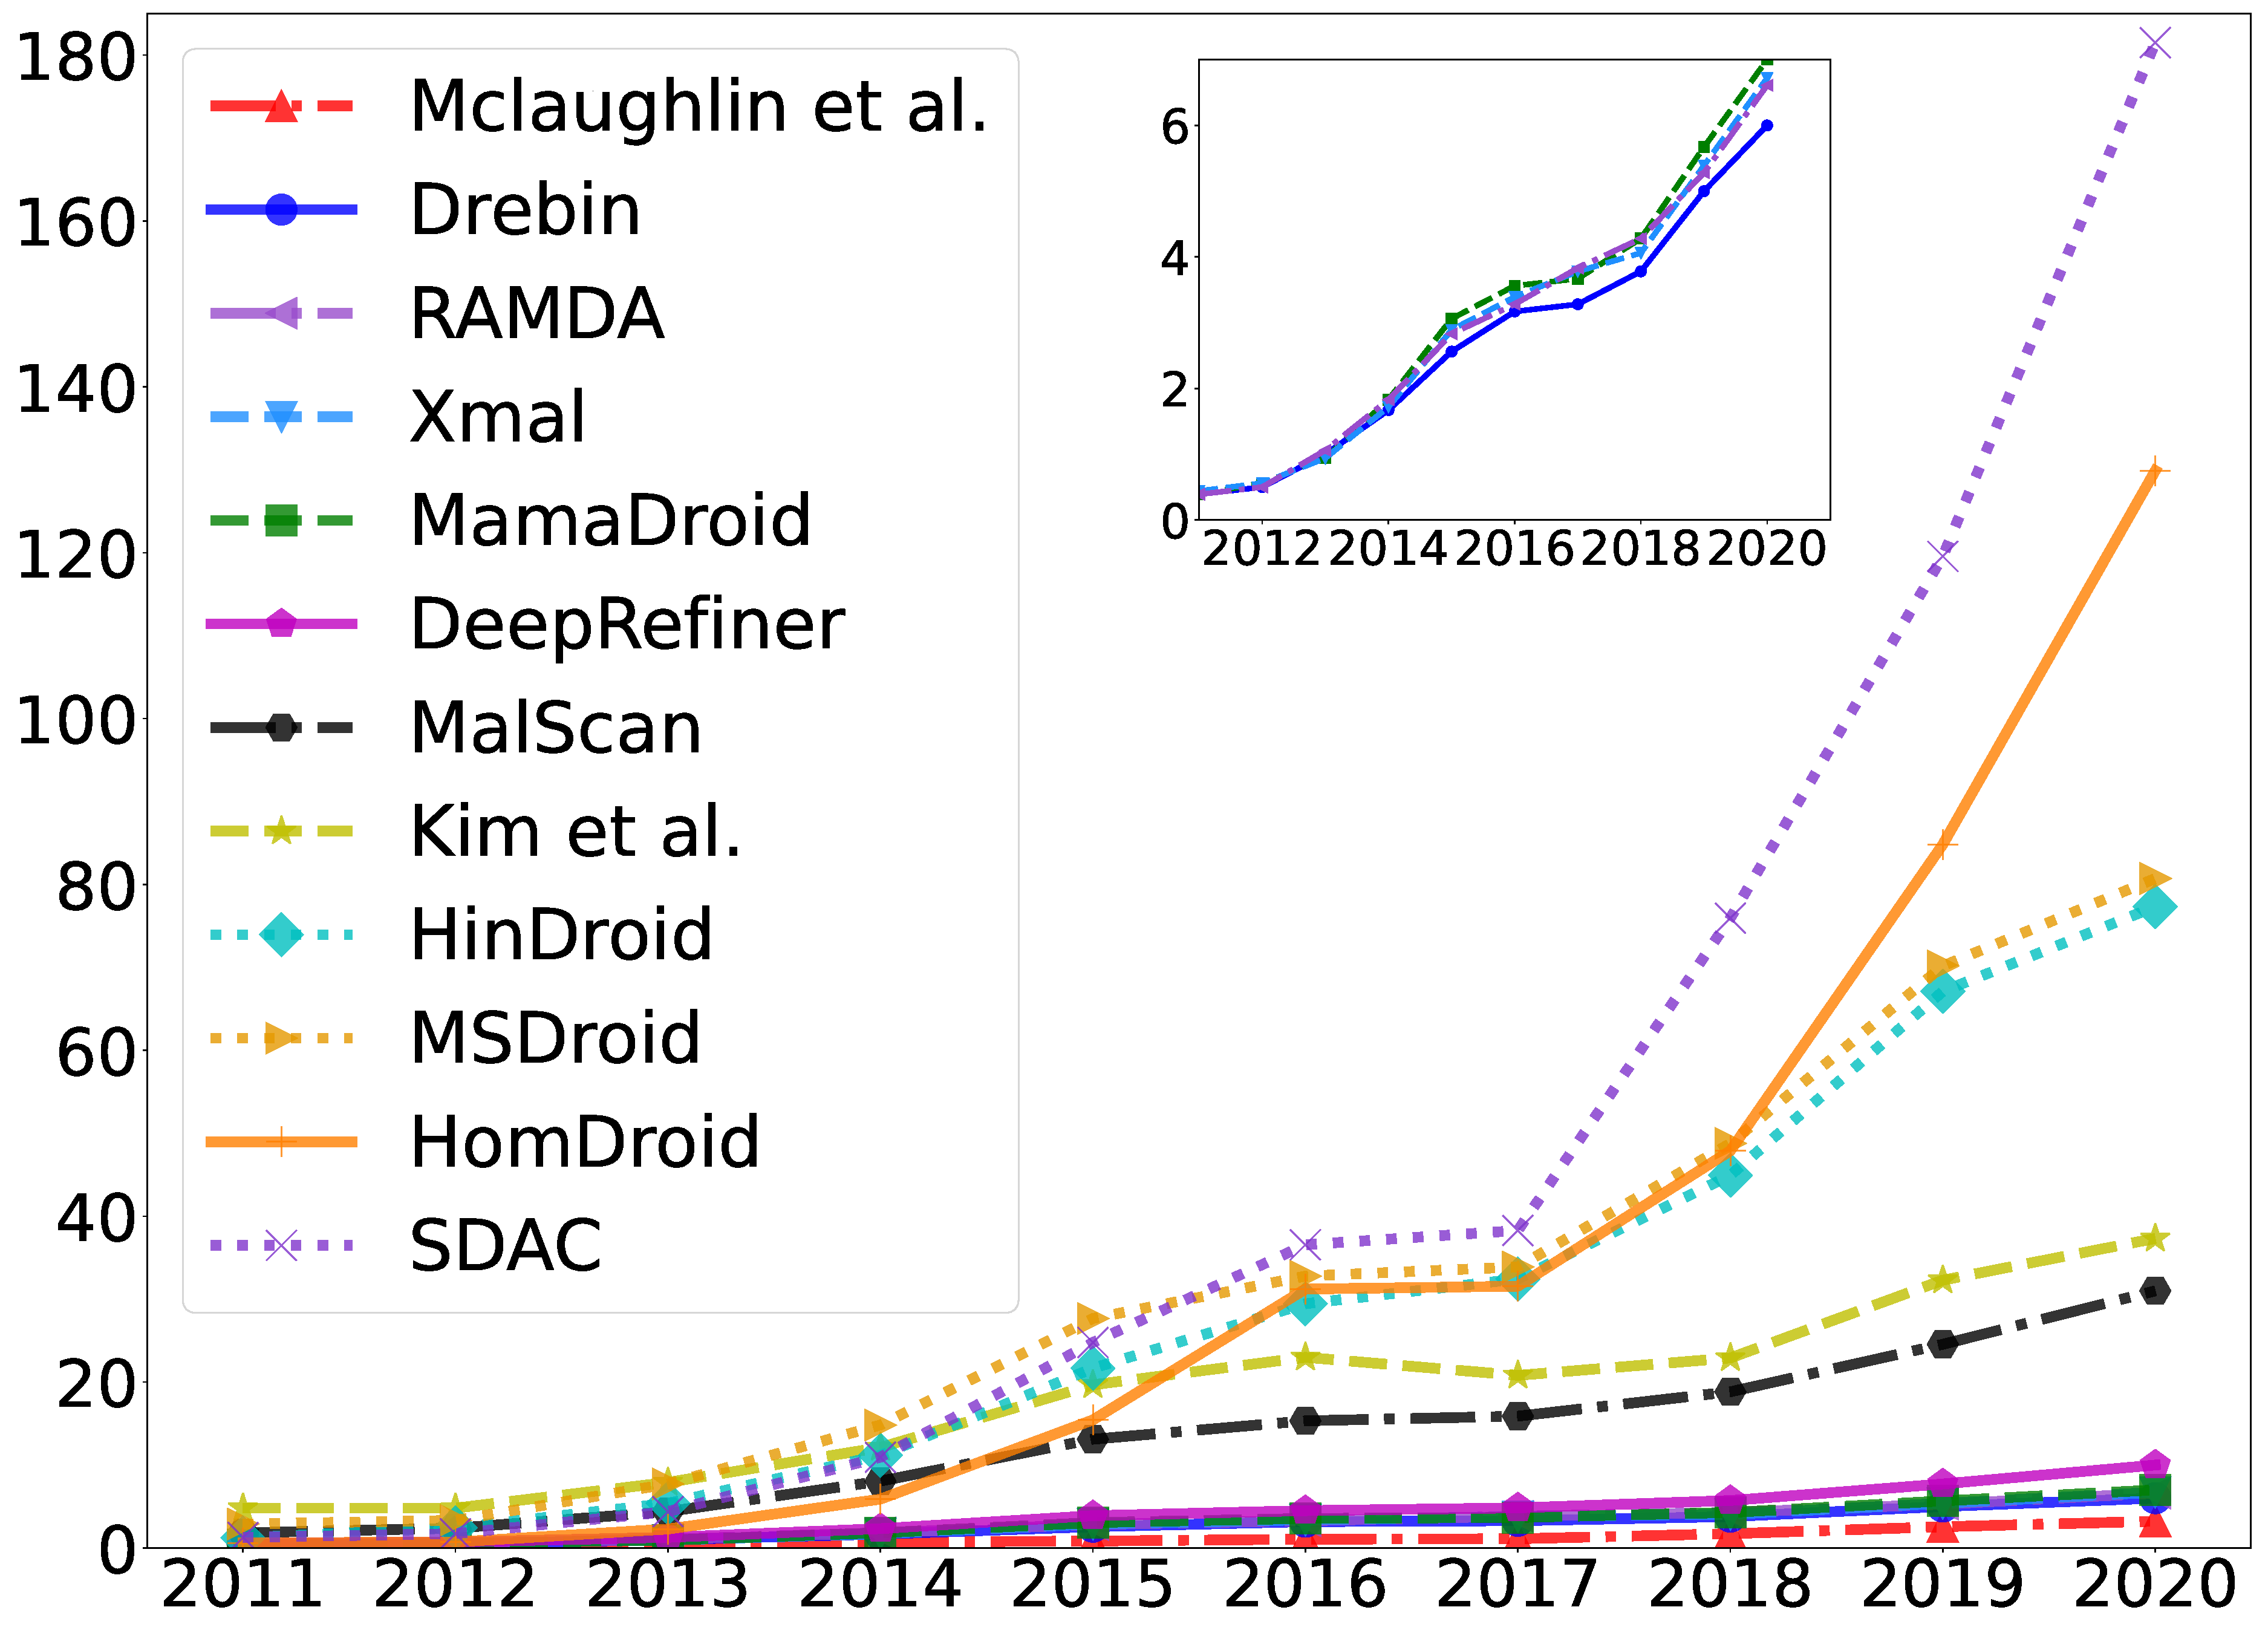
\includegraphics[width=0.56\linewidth]{fig/efficiency_encoding.pdf}
    % \vspace{-0.2cm}
    \caption{The efficiency of feature transformation of the selected approaches. The x-axis shows the dataset year, and the y-axis indicates the utilized time in hours.}
    \label{fig:efficiency_encoding}
    \vspace{-0.3cm}
\end{figure}

\begin{conclusionbox}
    \textit{Summary:}
    The efficiency of ML-based malware detectors does not positively correlated with their effectiveness. Finding a balance between these two aspects is crucial when developing new detectors, requiring careful alignment of feature semantics with model capabilities to achieve an optimal trade-off.
\end{conclusionbox}

\subsection{Further Experimental Validation}
\label{further_experiments}

\subsubsection{\textbf{Influence of Reverse Engineering Tools}}
\label{tool_influence}

\tosem{use APK tool to handle maybe 4000 apps, and then extract specific features, to test the influence of features for specific models (such as MLP, RF, SVM,...)
with new experiments dataset.}

\subsubsection{\textbf{Detection Effectiveness}}
\label{sec:detect_effectiveness}

\tosem{add the experiments year by year, to say the result is stable.
add 21-24 data, and re-run some experiments (effectiveness, evolution)}

\subsubsection{\textbf{Detection Efficiency}}
\label{sec:detect_efficiency}

\tosem{discuss the efficiency metrics, and add new efficiency metrics, and add new experiments}